\documentclass[aps,prl,10pt,twocolumn,floatfix]{revtex4-2}
\usepackage{chngpage}
\usepackage{graphicx}
\usepackage{dcolumn}
\newcolumntype{d}{D{.}{.}{-1}}
\usepackage{url}
\usepackage{amsmath}
\usepackage[version=3]{mhchem}
\usepackage{graphicx}
\usepackage{esvect}
\usepackage{circuitikz}
\usepackage{physics}

\bibliographystyle{apsrev4-2}


\begin{document}

\begin{abstract}
%What is the motivation?
%What did you   do?
%What were the results?
%Conclusion
\end{abstract}


\title{Lab \#1: Bainbridge Tube Measurement of E/M}
\author{Corbin T. Rochelle (ctr233)}
\date{\today}
\affiliation{Department of Physics and Astronomy\\Mississippi State University\\Mississippi State, MS 39762-5167}
\date{\today}

\maketitle

\section{Introduction}\label{Intro}

The purpose of the Bainbridge Experiment is to experimentally determine the charge-to-mass ratio of the electron.
This is done by observing a beam of electrons as they travel in an arc due to the presence of a magnetic field\cite{WingerBain}.
The diameter of the arc observed in the vacuum tube depends on how the charged electrons where affected by the magnetic field produced by a pair of Helmholtz coils to change its momentum.
By measuring the current in the Helmholtz coils to bend the electron beam to known diameters for a set acceleration voltages, the charge-to-mass ratio of the electron can be determined as will be shown later.

In 1897, J.J.~Thomson published a paper covering his experiments with cathode rays.
In his paper, Thomson stated that the ``unanimous opinion of German physicists [is that] they are due to some process in the aether" \cite{CathodeRays}.
This aether, one popular theory at the time for explaining how information could travel through vacuum, was laid as an explanation for the bending of the cathode rays shot from the filament in cathode ray tubes due to the magnetic field.
However, in his paper, J.J.~Thomson relays that people should examine the possibility of an unknown negatively charged particle, not as a ray manipulated by the aether.
In the latter sections of his paper he presented results from his experiments ``to test some of the consequences of the electrified-particle theory" \cite{CathodeRays}.

Thomson concluded through his experimentation that the $m/e$ ratio's average was  $1.29(17)\!\times\!10^{-7} kg/C$, which is in the units that he used at the time, which are different from the units used today.
He concluded that ``the smallness of m/e may be due to the smallness of m or the largeness of e, or to a combination
of these two;"
although he knew his experimental data to not know the true $m/e$ ratio, due to the variance in his data, he correctly concluded that ``its value is very small compared with the value, which is\ldots the value for the hydrogen ion in electrolysis" \cite{CathodeRays}.
Thomson came back later in 1913 and ran another experiment where he found a closer approximation to our current e/m amount \cite{Wiki}.

Kenneth Bainbridge was a scientist in the 20th century who, among other things, created the device students use in this lab while he was at Harvard \cite{Bainbridge}.
He published this lab in \textit{The Physics Laboratories}, entitled \textit{The Specific Charge of an Electron} \cite{Bainbridge}.
Bainbridge, in 1938, developed what we now know today as the Bainbridge Tube Measurement of $e/m$, which was not originally designed for scientists to use, but for students to use to develop skills for labs and experimental procedure \cite{Bainbridge}.
A version of his experiment is the basis for this lab report.


\section{Theory}\label{Theory}
\subsection{Derivation of Charge-to-Mass Ratio}
% Derivation of EQ1
The most important equation to determine the charge-to-mass ratio of the electron is
\begin{equation}\label{pears}
\frac{e}{m}=\frac{2V_{acc}}{r^2B^2}
\end{equation}
Since it is such an important equation I will now go through its derivation. \\
We begin with the Lorentz force
\begin{equation}
\va{F}=q(\va{E}+\va{v}\times \va{B})
\end{equation}
Since we know there is not an electric field applied to the electrons within the tube, $\va{E}$ goes to 0, meaning the new equation is
\begin{equation*}
\va{F}=q(\va{v}\times \va{B})
\end{equation*}
Now we introduce a second equation, the one for the centripetal force, given by
\begin{equation*}
\va{F}=-m\frac{\va{v}^2}{r}
\end{equation*}
We know that both of the these forces are causing circular motion.
So we conclude that these forces must be related to each other;
therefore we use Newton's Second Law of Motion to obtain
\begin{equation}\label{apples}
q(\va{v}\times \va{B})=m\frac{\va{v}^2}{r}
\end{equation}
Here we want to massively simplify the problem through the setup of the experiment, with the goal of representing $\va{v}\times \va{B}$ as $vB$.
The first choice is to use the Helmholtz coils instead of the anything else to create the magnetic field due to the stability and uniformity of the field the coils create.
We want the magnetic field to be constant throughout the vacuum, and this creates that.
We then have to consider that the magnetic field created by the Helmholtz coils is not the only $\va{B}$ field present.
We also must account for the Earth's magnetic field, which can easily be eliminated.
We do this by orienting the experiment in a specific vertical and horizontal orientation that aligns with Earth's $\va{B}$ field so we can negate its affects.
We can now include these adjustments to the experiment and solve for the velocity in equation \ref{apples} to obtain
\begin{equation}\label{oranges}
v=\frac{qBr}{m}
\end{equation}
Let us introduce the last needed equation, that for the kinetic energy of the electron beam in terms of the initial electrostatic potential energy of the electrons at the cathod given by
\begin{equation}
\frac{1}{2}mv^2=eV
\end{equation}
Substituting the velocity derived in equation \ref{oranges} yields
\begin{equation*}
\frac{1}{2}m(\frac{qBr}{m})^2=eV
\end{equation*}
which is rearranged to obtain the final expression of
\begin{equation}\label{blueberries}
\frac{e}{m}=\frac{2V_{acc}}{r^2B^2}
\end{equation}

\subsection{Linearization of Equation \ref{pears}}
% Linearization of Eq1 and 2
Starting with the equation for the magnetic fields of the apparatus and the Earth
\begin{equation}\label{dragonfruit}
B=B_0I-B_E
\end{equation}
Substituting equation \ref{dragonfruit} in for the equation \ref{pears} gives
\begin{equation*}\label{papaya}
\frac{e}{m}=\frac{2V_{acc}}{r^2(B_0I-B_E)^2}
\end{equation*}
Since the dependent variable we are looking for is the current, we  solve equation \ref{papaya} to obtain
\begin{equation}
I=\frac{\sqrt{2m}}{B_0\sqrt{e}}\cdot \frac{\sqrt{V_{acc}}}{r}+\frac{B_E}{B_0}
\end{equation}
In this final equation, we can clearly see the independent and dependent variables.
\subsection{Questions}
% Answering Questions
Which part of the beam should hit the post? I.e., what is the effect on the beam of hitting the gas
molecules in the tube?\\
The part of the beam that should hit the post is the very outer edge because this is the part of the beam that carries the most energy, most closely approximating the energy the entire beam had at its inception.
This is because the beam of light created before the post is using the outer, most energetic electrons, which when imparting their energy on the Mercury gas, lose some of their initial energy and fall into the middle of the beam.
Since the electrons that have interacted with the Mercury atoms have lost some initial energy we do not want to use these in our measurements, so we use the new fresh outer electrons at the post.

How do maximize the range over which data can be taken? What are the experimental conditions that
set the minimum and maximum data point?\\
We maximize and minimize the range over which data can be taken by varying the voltage of $V_{acc}$, this moves the beam in and out with respect to the posts inside the glass tube.
The experimental conditions that set the minimum and maximum data points in this experiment are the posts in the glass tube.
They give a frame of reference for which to measure the radius of the beam of electrons.
The minimum voltage is set by the fact you need to be able to see the beam at the farthest point in order to obtain the bending current, At lower acceleration voltages, the beam may not reach the post or the path is too dim to observe. For the maximum voltage, there is a limit set by the maximum current which can be sent through the Helmholtz coils to bend the beam to the first post.

What is the optimal way to analyze the data set so that all data points are treated properly?\\
The optimal way to analyze the data set so that all of the data is analyzed properly is to linearize the data set and then use a linear regression to find the relation between data points.
This is because linear plots are much easier to analyze to check for relations when compared to other types of relations.
Another thing to keep track of are the systematic uncertainties due to the way the experiment was preformed.

\section{Experiment}
% about device
The device we used for this experiment was the Bainbridge tube.
The basics of the device are two Helmholtz coils, a glass tube filled with mercury gas, and an anode that electrons are shot from.
Once connected to a power supply, and set to the correct amperage and voltage, electrons will be shot from the anode and make a loop, because of the Lorentz force.
The electrons, traveling in the tube, will collide with the mercury gas, imparting energy to it, lighting it up.
Figure \ref{bain} gives a less theoretical, more applicable interpretation of the construction of the Bainbridge Apparatus.
\begin{figure}\label{bain}
    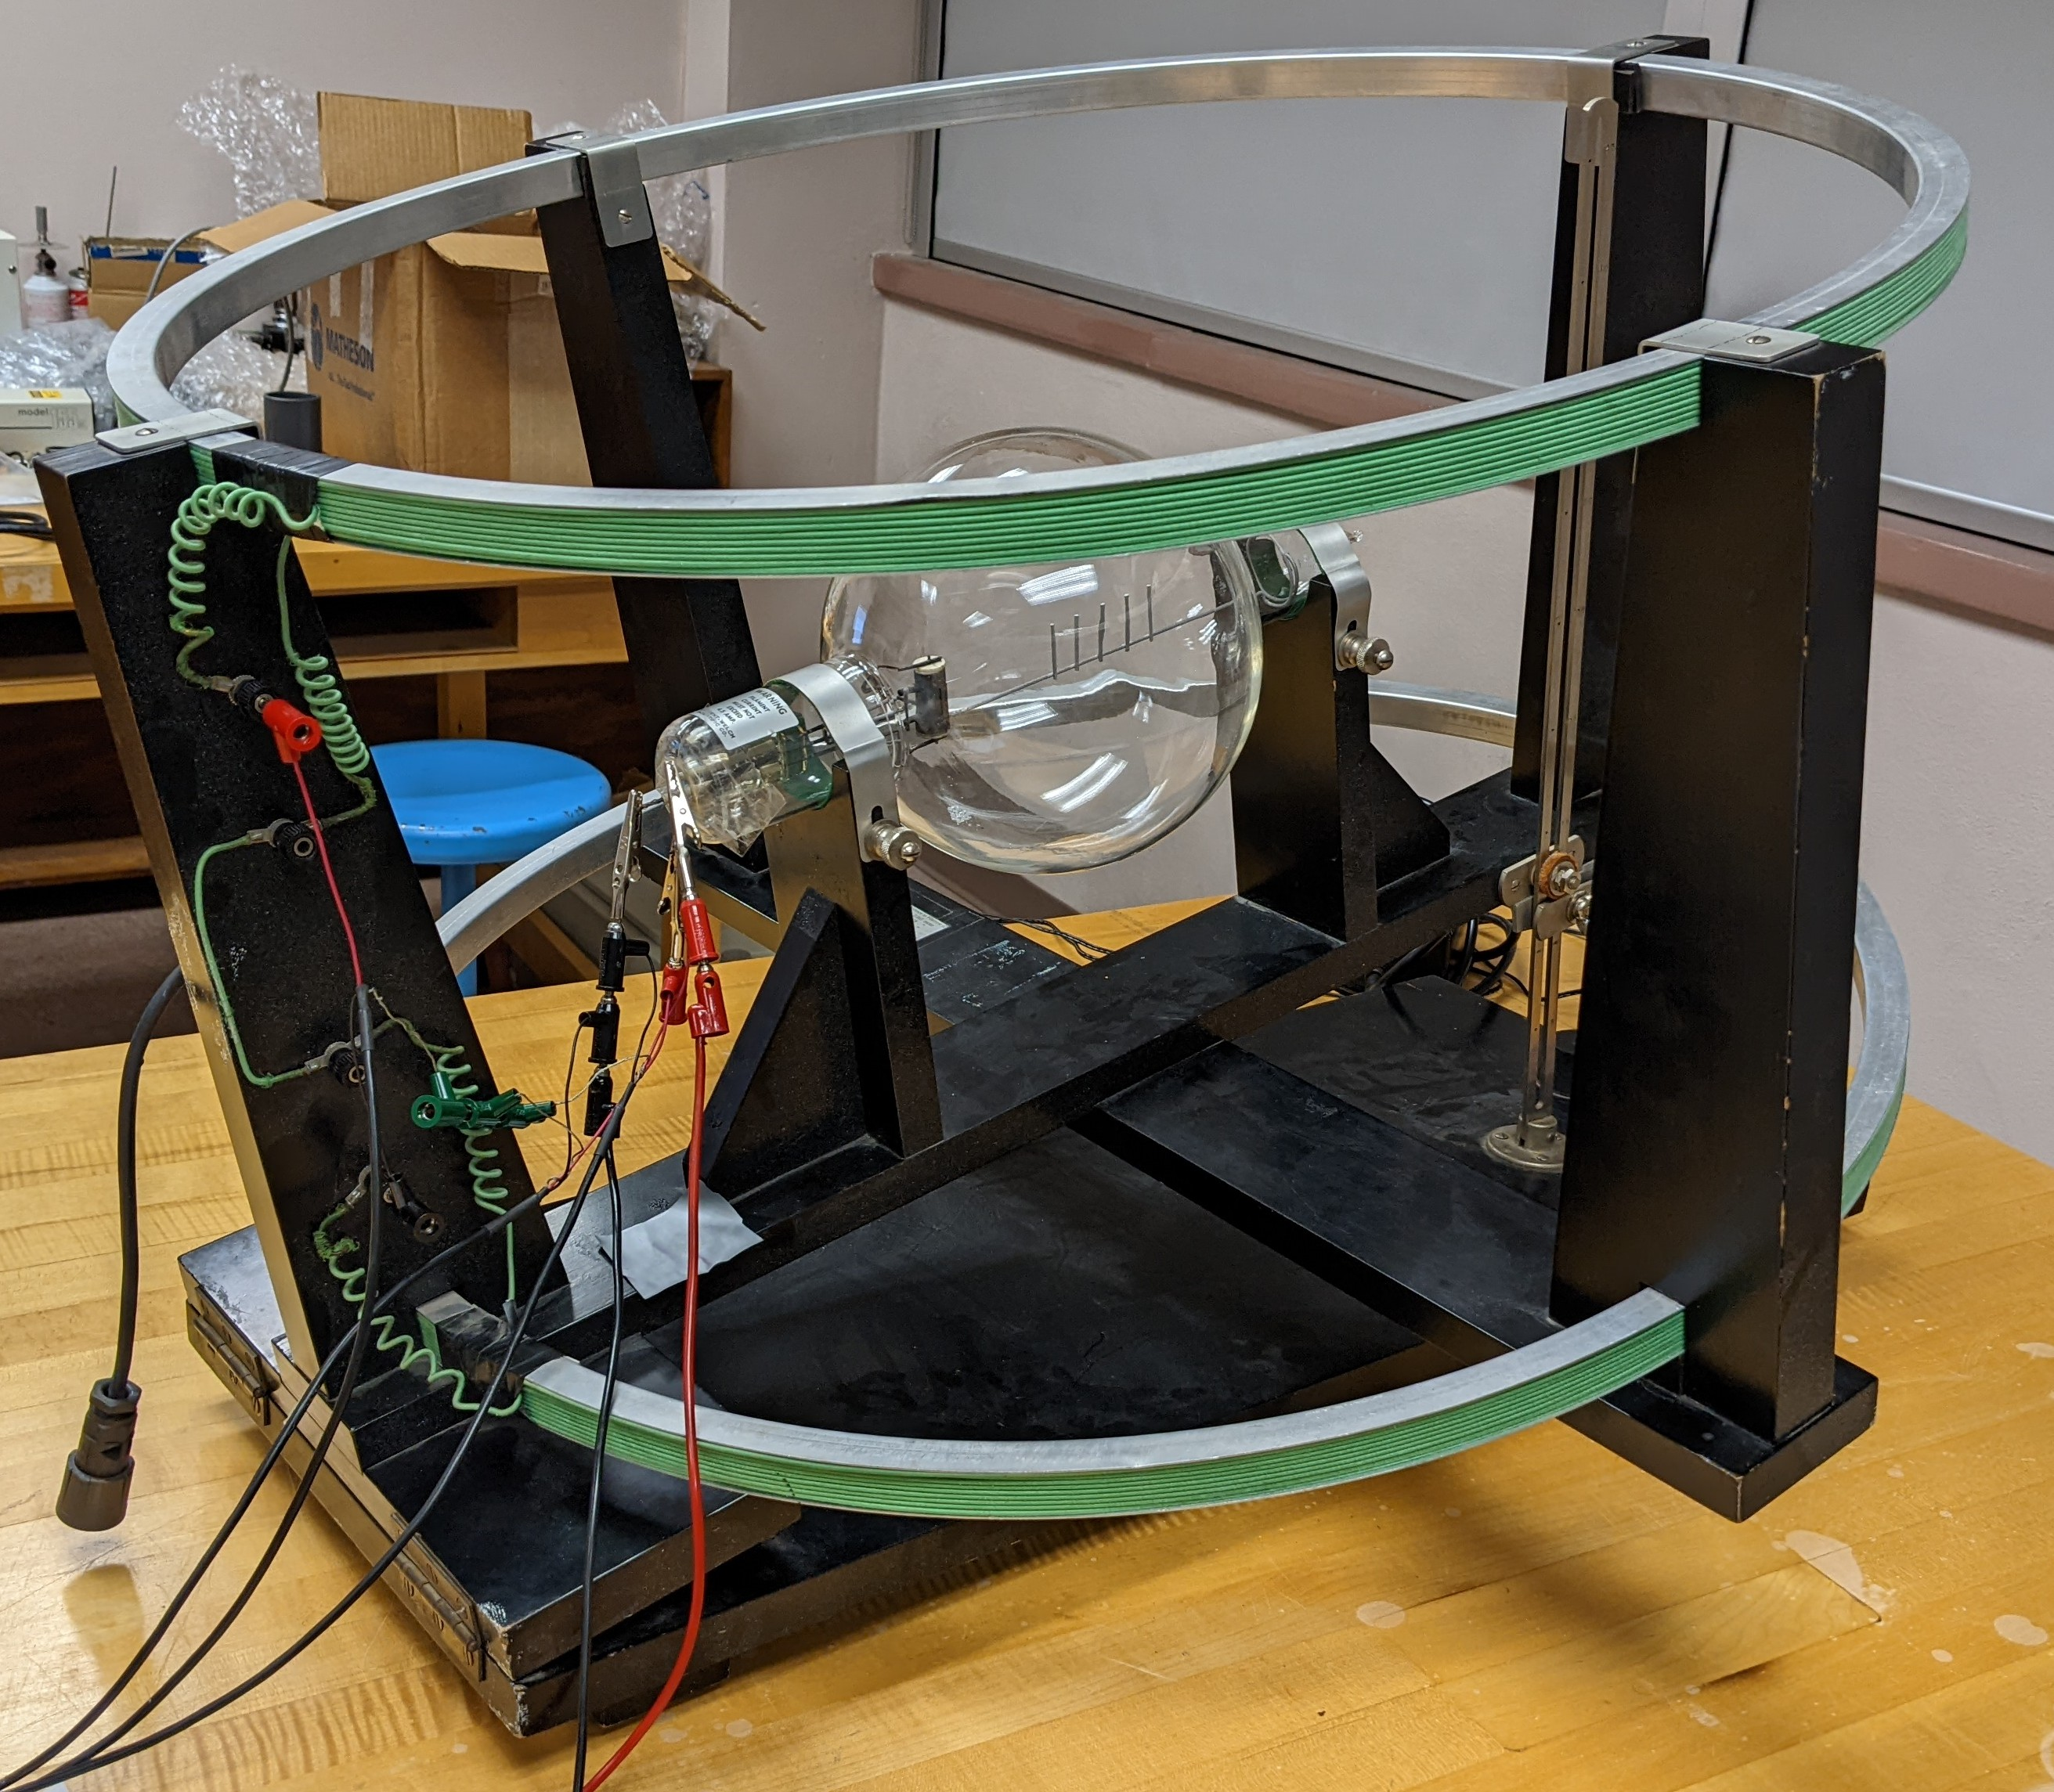
\includegraphics[width=230px]{bain.jpeg}
    \caption{A Picture of the Bainbridge Apparatus}
\end{figure}
% what you did
The data collection was broken up among eight different groups of two students.
Each group was assigned two acceleration voltages and each group member recorded the current it took to reach each post at that given voltage for the other.
After collecting all of the data, the post measurements were found in the Bainbridge lab manual and data analysis could begin.
% Set up
Setting up the Bainbridge Experiment was one of the most important steps in this entire experiment.
There were two important steps: aligning parallel to the Earth's magnetic field and getting the bulb rotated.
% electric field
There were two steps involved in aligning to Earth's magnetic field, that is aligning on our horizontal axis first, and then on our vertical axis.
To align the horizontal axis, firstly we placed the Bainbridge apparatus on a table and a dip needle oriented horizontally was placed in near proximity to the device.
Using the compass, we oriented the bulb's ends along the magnetic field lines.
Next, the dip needle was rotated into a vertical orientation and the North end of the Bainbridge apparatus was raised to align the axis of the Helmholtz coils with the Earth's magnetic field.
This alignment was performed to satisfy the requirements for the net magnetic field as descried in theory section.
% bulb rotation
The last step in alignment of the setup was to rotate the bulb so that the election beam was perfectly perpendicular to the magnetic field of the Helmholtz coils, as to create a circle instead of a helix.
This is important so that the beam of electrons hits the posts exactly at the perpendicular angle as to get rid of all energy lost due to motion in the y direction.
%observations
During the experiment, we observed exactly what we thought would happen, the Helmholtz coils induced a curl in the electron beam, that excited the mercury gas.
With the lights off, we could clearly see a ring of electrons illuminating the gas.


\section{Data Analysis}
%Data
For this data analysis, we used a linear regression using Gaussian statistics, specifically Chi-Squared Minimization.
For the linear regression, formed by the Chi-Squared Minimization, we obtained a slope, that is designated in these formulas as $a_0$.
The value for $a_0=0.0173753$.

%Figure
\begin{figure}
    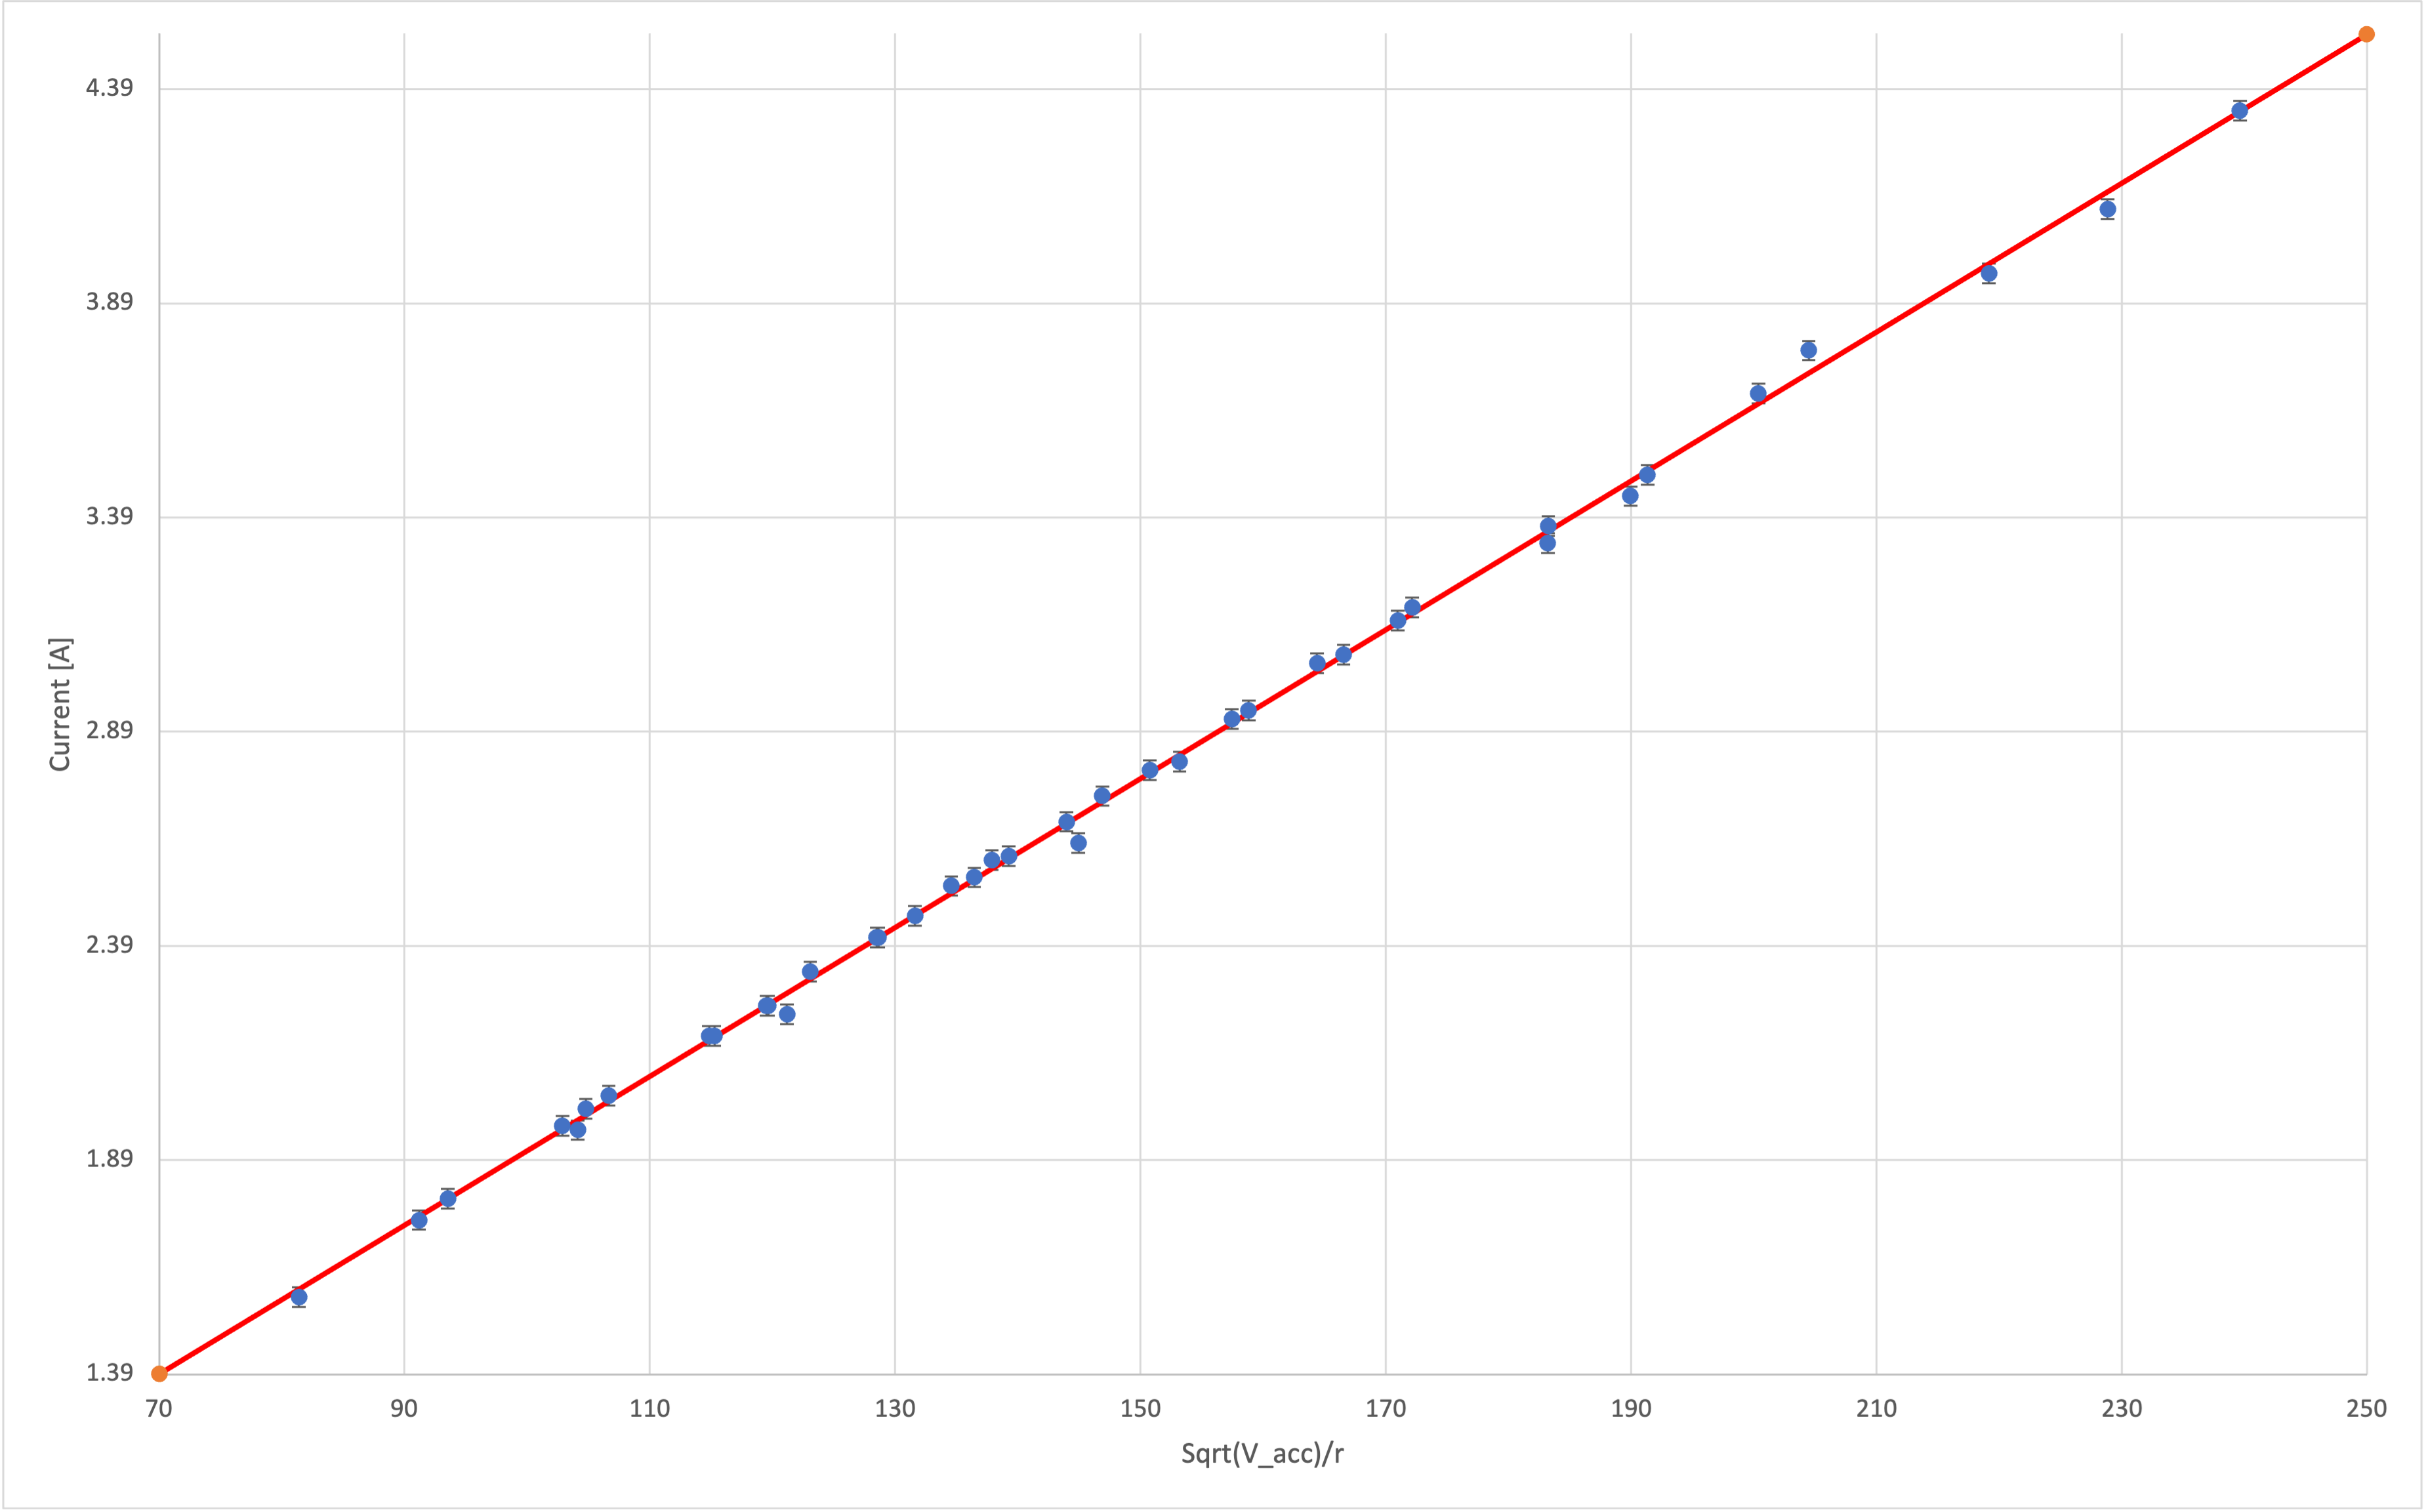
\includegraphics[width=230px]{data_plot.png}
    \caption{A Plot of Current vs the Square Root of Acceleration Voltage Over Radius}
\end{figure}

%e/m ratio from data
To find the charge-to-mass ratio of the electrons, we simply use Equation \ref{pears}, along with the equation for the magnetic field, given by
\begin{equation}
	\va{B_0}=\frac{8\mu_0N}{\sqrt{125}a}=195.178 T
\end{equation}
where $\mu_0$, $N$, and $a$ are all constants given as $1.256637\frac{\mu m\cdot kg}{s^2A^2}$, 72, and $0.3317m$ respectively.
We then plug this value of $B_0$ into
\begin{equation}
	\frac{e}{m}=\frac{2}{(a_0B_0)^2}=1.73908\cdot10^{11}\frac{C}{kg}
\end{equation}


\section{Conclusion}
% how does it compare to current science
The current accepted charge-to-mass ratio of the electron is $1.758820\cdot10^{11}\frac{C}{kg}$, so the \% error is
\begin{equation}
	\frac{1.758820\cdot10^{11}}{1.73908\cdot10^{11}} -1=0.011308\%
\end{equation}
From this \% error we can see that the value we obtained in the lab is very close to the current accepted value for the charge-to-mass ratio of the electron. 
The standard deviation I obtained from the data was $0.198$, so my values is within one, let alone two, standard deviations of the data. 

\begin{thebibliography}{9}
\bibitem{WingerBain} J. ~Winger, \textit{Bainbridge Tube Measurement of e/m}, (Mississippi State University).
\bibitem{CathodeRays} J. J. ~Thomson, \textit{Cathode Rays}, (Philosophical Magazine, 1897).
\bibitem{Wiki} J.J. ~Thomson, \textit{Rays of Positive Electricity}, (Proceedings of the Royl Society, 1913).
\bibitem{Bainbridge} K. T. ~Bainbridge, \textit{The Specific Charge of the Electron}, (American Journal of Physics, 1938).
\end{thebibliography}

\end{document}
